The proposed solution has three phases and uses four techniques described in detail in sections 5,6,7 and 8. The first phase is the setup phase, whose goal is to provide the holder with the necessary keys to participate in the protocol. The second phase is the issuing phase, where the Issuer issues a credential to the Holder. The third and last phase is the presentation phase, where the Holder presents one or several credentials to the Verifier.

During the setup phase, the user is required to register his secret encryption key ($mk$) with a key escrow service. In response, the key escrow service issues multiple public keys ($pk_i$) corresponding to the same secret key, with each of these public keys digitally signed ($\sigma_i$) by the key escrow service. In addition to the act of signing these public keys, the key escrow service also guarantees the provision of revocable anonymity for holders who engage in malicious or improper behavior.

\begin{figure}
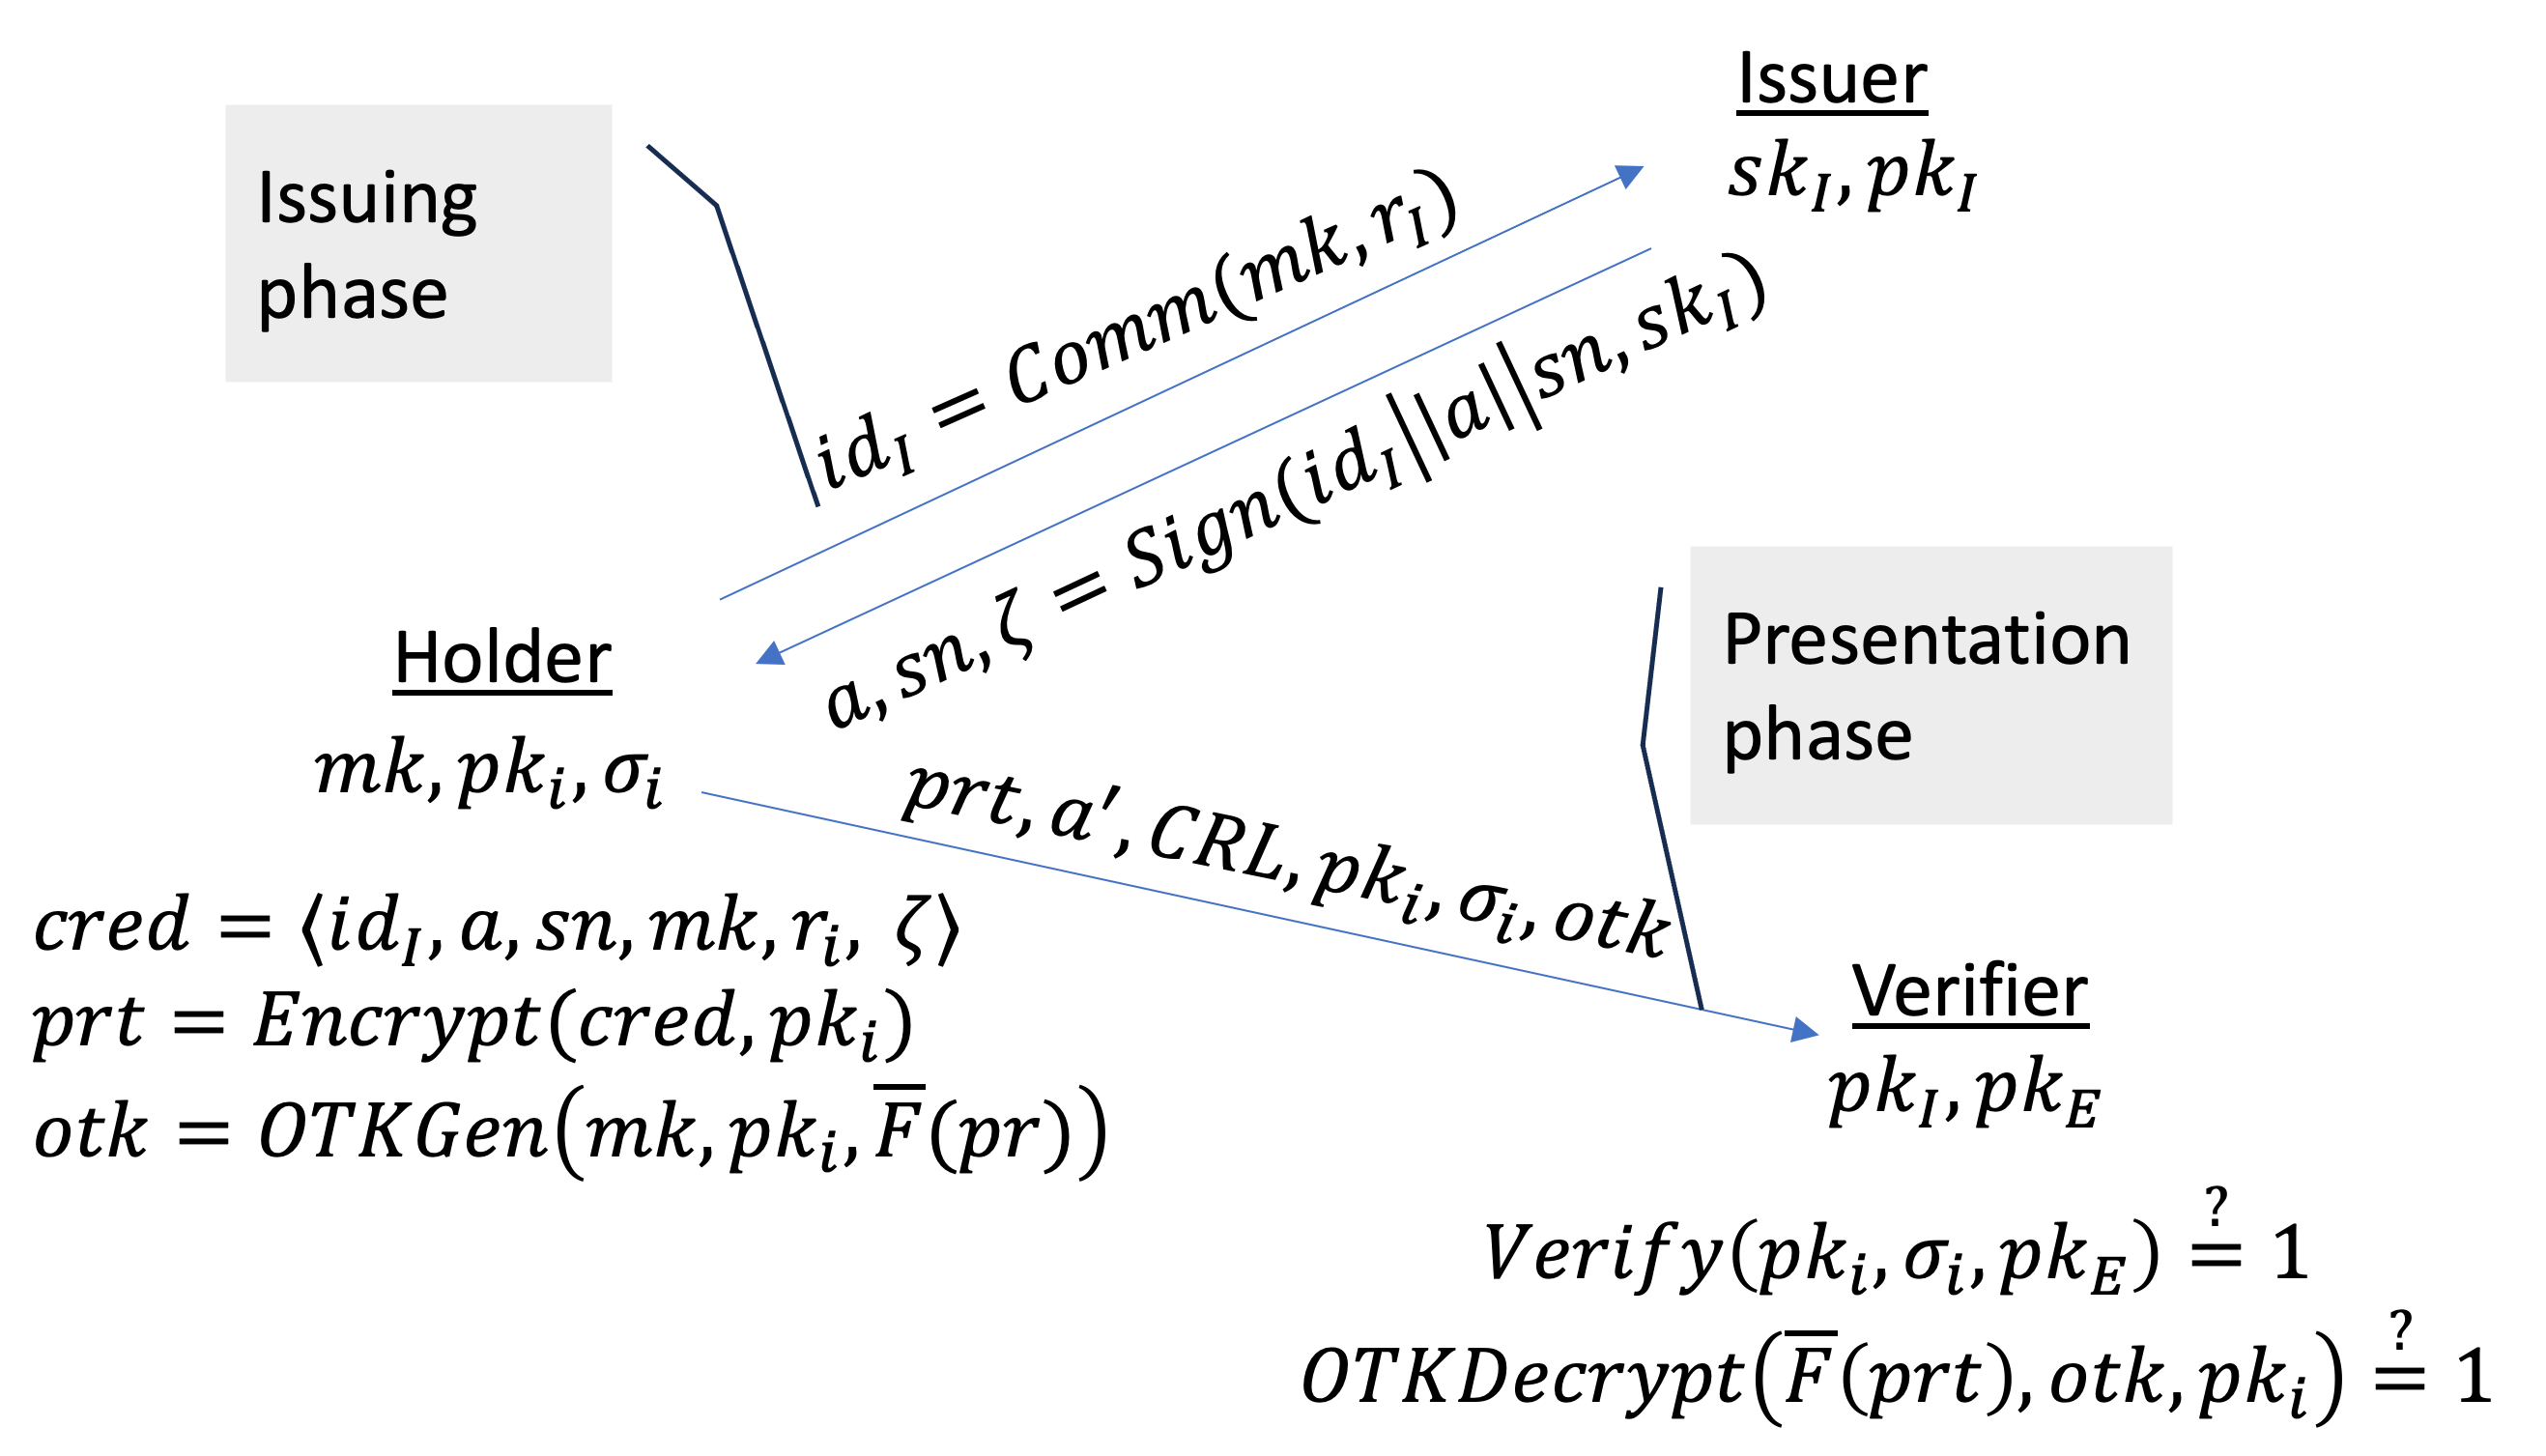
\includegraphics[width=\columnwidth]{schema.png}
\caption{Issuing and presentation phases of the proposed solution.}
\label{fig:schema}
\end{figure}

The issuing phase (cf. Figure \ref{fig:schema}) starts with the holder committing to her secret key ($mk$) while introducing an element of randomness ($r_I$). Subsequently, she uses this commitment $id_I=\bkw{Comm}(mk,r)$ as her unique identifier for a specific issuer $I$. The issuer, in turn, takes the commitment $id_I$, some attributes of the holder $a$ and the serial number $sn$ of the credential, signs all with the issuer's secret key $sk_I$ and returns the signature $\varsigma=\bkw{Sign}(id_I\|a\|sn,sk_I)$, the attributes $a$ and the $sn$ number back to the holder.

In the presentation phase (cf. Figure \ref{fig:schema}), the holder encrypts the credential $cred =\langle id_I, a,  sn, mk, r_i, \varsigma\rangle$, with a homomorphic encryption algorithm and one of her public keys $pk_i$. 

Then, the holder sends the presentation message, with:
\begin{itemize}[noitemsep]
\item The resulting presentation ciphertext $prt = \bkw{Encrypt}(cred,pk_i)$,
\item The holder's attributes to be revealed $a'$ (not necessarily the attributes $a$ in the credential $cred$),
\item The public key $pk_i$ used to encrypt the credential and the correspondent signature from the escrow service $\sigma_i$,
\item A decryption key $otk=\bkw{OTKGen}(mk,pk_i,\overline{F}(prt))$ that can only be used to decrypt a specific homomorphic computation $\overline{F}(prt)$ over the presentation ciphertext $prt$, and
\item A certificate revocation list $CRL$ containing the serial numbers of revoked credentials (which could also be taken from someplace else, e.g. a distributed ledger).
\end{itemize}

The function $\bkw{OTKGen}$ generates a special decryption key $otk$ that allows the delegation of the decryption of a specific ciphertext to the verifier without delegating the decryption of all ciphertext encrypted with the same key. (cf. Section \ref{sec:otk}).

Upon receiving the presentation message, the verifier:
\begin{itemize}[noitemsep]
\item Checks the signature $\sigma_i$ on the public key $pk_i$ of the holder,
\item Recomputes and decrypts $\overline{F}(prt)$, with the $otk$ and the holder's public key,  and checks if the result is valid \[\bkw{OTKDecrypt}(\overline{F}(prt),otk,pk_i)\stackrel{?}{=}1\]
\end{itemize}

The homomorphic computation $\overline{F}(prt)$ that both the holder and the verifier must perform on the encrypted credential $prt$, is the conjunction of four elements $\overline{F}(prt) = prt_{oc} \wedge prt_v \wedge prt_{CRL} \wedge prt_a$, each of them being the result of a specific homomorphic test (see Table \ref{tab:hcomp}).
The first test $prt_{oc}$ checks that the user owns the commitment $id_I$, opening the commitment with the secret key of the holder $mk$ and the randomness $r_I$ used to create the commitment. The second test $prt_v$ checks the signature of the credential with the public key of the issuer $pk_I$. The third test $prt_{CRL}$ checks that the credential serial number is not in the issuer's CRL, and finally the last test $prt_a$ checks that the derived attributes $a'$ are consistent with the signed attributes $a$. The homomorphic test $\overline{Check}$ depends on the specific attributes $a$ and $a'$, for example, if $a$ contains an address with an EU member state and the holder wants to prove that that address is from an EU member state, it can be implemented with the ``Private Set Membership'' primitive $\overline{\bkw{PSM}}(prt,EU)$, which tests that the member state in the address is one of the EU member states, without revealing the member state in the address. 

\begin{table}[ht]
    \renewcommand*{\arraystretch}{1.3}
    \centering
    \begin{tabular}{l|l|l}\hline
         Element & Homo. Test & Result \\\hline
         $prt_{oc}$ & $\overline{\bkw{OpenCom}}(prt)$ & $\senc{\bkw{OpenCom}(id_I,mk,r_I)}{pk_i}$ \\\hline
         $prt_{v}$ & $\overline{\bkw{Verify}}(prt,pk_I)$ & $\senc{\bkw{Verify}(id_I \|a\|sn,\varsigma,pk_I)}{pk_i}$\\\hline
         $prt_{CRL}$ & $\overline{\bkw{PSM}}(prt,CRL)$ & $\senc{sn \notin CRL}{pk_i}$\\\hline
         $prt_a$ & $\overline{Check}(prt,a')$ & $\senc{Check(a,a')}{pk_i}$\\\hline
    \end{tabular}
    \caption{Homomorphic tests performed over the credential presentation.}
    \label{tab:hcomp}
\end{table}

Note that the credential presentation is not traceable by any combination of verifiers and issuers because it is always a fresh encryption and the encrypted values are never revealed to the verifier. 

The following section introduces some background and notation required by the remaining sections, which describe each of the previously used primitives. Section \ref{sec:otk} describes the primitives $\bkw{Encrypt},\bkw{OTKGen}$, and $\bkw{OTKDecrypt}$, while the primitive $\overline{\bkw{PSM}}$ is described in Section \ref{sec:comparison}. Section \ref{sec:owner} describes the primitives $\bkw{Comm}$, $\bkw{OpenCom}$ and $\overline{\bkw{OpenCom}}$, and the primitives $\bkw{Sign}$, $\bkw{Verify}$, and $\overline{\bkw{Verify}}$ are described in Section \ref{sec:sig}.
